\documentclass[a4paper,12pt]{book}
\usepackage[utf8]{inputenc}
\input apl.tex

\usepackage{mathtools}
\usepackage{cancel}
\usepackage{applekeys}
\usepackage{graphicx}
\usepackage{keystroke}
\usepackage{menukeys}
\usepackage{amsmath}
\usepackage{amssymb}
\usepackage[english]{babel}
\usepackage{upquote}
\usepackage{wrapfig}
\usepackage{makeidx}

\usepackage{fancyvrb}
\usepackage{listings}
\usepackage[margin=2cm]{geometry}

\makeindex

\title{\large Avril APL\\
{\normalsize (Content not (yet) checked for grammar and spelling errors)}}
\author{Eduardo Costa \and Marcus}
\date{}

%\begin{lstlisting}[escapechar=+]
%  bla, bla,
%  bla +$\leftarrow$+
%\end{lstlisting}

\newcommand{\reduce}{$/\!\!\!\textendash$}
\newcommand{\cancelequiv}{$/\!\!\!\!\!\equiv$}
\newcommand{\nspc}{$\:\!\:\!\!\!\!\!\!\!$}

\lstdefinelanguage{apl}
{
morekeywords={←,⍴,⍺, ⍵, ⎕, ÷, ×,
  ≢, ∆, ⌿, ∧, ⊢, ∘, ○,
  ⌊, ⌈, ⍳, ⍕},
otherkeywords={:cmd},
keywordstyle=\bfseries,
sensitive=\true,
breaklines=\true,
literate=
{←}{$\leftarrow{}$}{1}
{⎕}{$\square{}$}{1}
{:cmd}{\cmdkey{}}{0}
{⍴}{$\rho$}{2}
{⍺}{$\alpha$}{1}
{⍵}{$\omega$}{1}
{÷}{$\div$}{2}
{⋄}{$\diamond$}{1}
{≢}{\cancelequiv}{2}
{∆}{$\Delta$}{1}
{⌿}{\reduce}{2}
{^}{$\&$}{1}
{⊢}{$\vdash$}{1}
{∘}{{\small $\circ$}}{1}
{○}{$\bigcirc$}{1}
{×}{$\times$}{1}
{⍳}{$\iota$}{1}
{⌊}{$\lfloor$}{1}
{⌈}{$\lceil$}{1}
{⍕}{$\top\nspc\circ$}{2},
morecomment=[l]{⍝}
}
\lstset{extendedchars=\true, upquote=\true, basicstyle=\ttfamily}
\lstset{aboveskip=\baselineskip, belowskip=\baselineskip}


\begin{document}
%% \maketitle
\begin{titlepage}
    \centering
    \vfill
    {\bfseries\Large
        Avril APL\\
        An introduction\\
        \vskip2cm
        Eduardo Costa\\
        Maybe Marcus Santos\\
    }    
    \vfill
    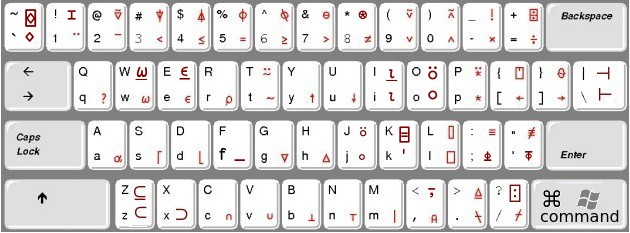
\includegraphics[width=15cm]{figs/apl-keyboard.jpg}
    \vfill
    \vfill
\end{titlepage}

\thispagestyle{empty}

\clearpage

\chapter{apl keyboard}
\pagenumbering{arabic} 
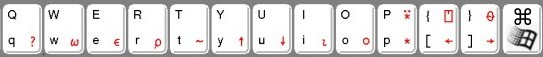
\includegraphics{figs/qwerty-row.jpg}

\large
The command key ~\cmdkey~ (win key)
is represented as \# in the comments.
To input ⍵, one should type \verb|#w|, i.e.,
hold the command key down and strike w.
In the figure above, it is the last key
on the right-hand side of the QWERTY row
of the keyboard.

\label{april:install}
\large
\begin{lstlisting}[language=apl]
~$ setxkbmap -layout us_intl,apl -option grp:win_switch
~$ rlwrap sbcl --noinform
CL-USER(1): (ql:quickload 'april :silent t)
(APRIL)
CL-USER(2): (in-package :april)

#<PACKAGE "APRIL">
APRIL(3): (april-f "V ← 3.4 8.5 9.2 4.0") ; #[ ←

#(3.4d0 8.5d0 9.2d0 4.0d0)
APRIL(4): (april-f "{+/⍵ ÷ ⍴ ⍵} V") ; #w⍵, #=÷, #r⍵
6.275000000
6.2749999999999995d0
APRIL(5): (cl-user::exit)
~$ 
\end{lstlisting}

\verb||\\
{\hspace*{-0.8cm}
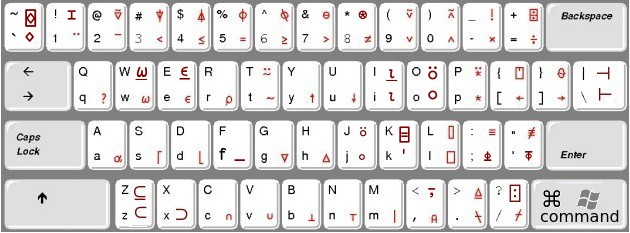
\includegraphics{figs/apl-keyboard.jpg}}
\label{april:keyboard}

On page~\pageref{april:install}, you gained insights into utilizing Quicklisp for loading April APL into Steel Bank Common Lisp (hereinafter referred to as sbcl). I assume you are already familiar with the installation process of sbcl and the configuration of Quicklisp.

After quickloading the \verb|'april| compiler,
I accessed its package using the
command \verb|(in-package :april)|. The following
command assigned a vectorial quantity to the variable \verb|V|:

\begin{lstlisting}[language=apl]
APRIL(3): (april-f "V ← 3.4 8.5 9.2 4.0")
\end{lstlisting}

In the sexpr \verb|(april-f "{+/⍵ ÷ ⍴ ⍵} V")|,
the subexpression \verb|{+/⍵ ÷ ⍴ ⍵}| represents a function that calculates the average of the elements of \verb|V|. The symbol ⍵ denotes the right-hand side argument of the function. The subexpression \verb|+/| inserts the \verb|+| operator between the elements of ⍵=\verb|V|, resulting in \verb|3.4+ 8.5+ 9.2+ 4.0|. Since ⍴⍵ calculates the length of ⍵, the entire expression computes the average.

Given that we are within the \verb|APRIL| package, attempting to exit using the sexpressions \verb|(exit)| or \verb|(quit)| proves ineffective for leaving SBCL. Consequently, it becomes essential to execute \verb|(cl-user::exit)|, prefixing the procedure \verb|exit| with the name of the package where it is defined.

To type APL programs, special characters are required. On GNU-Linux, the command below facilitates the inclusion of the APL set of symbols. Whenever you wish to work with APL, open a terminal and execute the \verb|setxkbmap| command.
\begin{verbatim}
~$ setxkbmap -layout us_intl,apl -option grp:win_switch
\end{verbatim}

\begin{wrapfigure}[3]{l}{1.5cm}

\includegraphics{figs/window-key.jpg}
\end{wrapfigure}
To type an APL symbol, one needs a prefix-key
for producing it. For this purpose, the option
\verb|grp:win_switch| selects the
command key~\cmdkey,
identifiable by the Microsoft Windows flag.

In the comments of page~\pageref{april:install},
the symbol \verb|#| denotes the command
key~\cmdkey~ as the prefix.
For instance, \verb|#w| (\cmdkey w) signifies
holding down the command key~\cmdkey~ and then pressing
the \verb|w| key to generate the APL symbol ⍵.
Similarly, \verb|#r| (\cmdkey r) indicates
that you should keep the window key pressed
and strike the \verb|r| key
to obtain the APL symbol ⍴.

\section{Star operator}
On page~\pageref{april:install}, you learned
how to calculate the average of the elements
in a vector. Listing~\ref{fig:star-operator}
shows how to calculate the standard deviation.

\begin{lstlisting}[language=apl, label={fig:star-operator},
                    caption={Standard Deviation}]
APRIL(8): (april-f "V← 4.5 8 3.6 12")

#(4.5d0 8 3.6d0 12)
APRIL(9): (april-f "{((+/(⍵ - +/⍵ ÷⍴⍵)*2)÷⍴⍵)*0.5} V")
3.309361721
#(3.3093617209365314d0)

%\caption{Standard Deviation}
%\label{fig:star-operator}
\end{lstlisting}


% 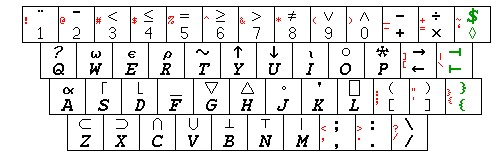
\includegraphics{figs/kb-apl-draw.jpg}

In listing~\ref{fig:star-operator}, the star
operator \verb|v * n| elevates \verb|v| to
the \verb|n-th| power. To obtain the star symbol,
you must type~\cmdkey p by holding down the win
key and striking \verb|p|. Below, you can
see what happens when one calculates \verb|X*2|,
where \verb|X| is a vector.
\begin{lstlisting}[language=apl]
APRIL(12): (april-f "X← 3 4 5 8")

#(3 4 5 8)
APRIL(13): (april-f "X * 2")
9 16 25 64
#(9 16 25 64)
\end{lstlisting}

The expression (⍵ - +/⍵ ÷ ⍴⍵) subtracts the
average of each element of the ⍵ right
hand side argument, where the average
is calculated by +/⍵ ÷ ⍴⍵ (see
page~\pageref{april:install}).
Therefore, (⍵ - +/⍵ ÷ ⍴⍵)*2 is a vector
whose elements are represented in
equation~\ref{eq1} as
$(\omega_i - \overline{\omega})^2$.

\begin{equation} \label{eq1}
  s = \sqrt{\frac{1}{N} \sum_{i=1}^N
         (\omega_i - \overline{\omega})^2}
\end{equation}

The expression /+(⍵ - +/⍵ ÷⍴⍵)*2 performs the summation
of the elements of (⍵ - +/⍵ ÷ ⍴⍵)*2.

Let us denote s as the expression
((+/(⍵ - +/⍵ ÷ ⍴⍵)*2) ÷ ⍴⍵).
Then s*0.5 elevates this
expression to the power of 0.5, which is
equivalent to extracting the square root:
\verb|{s←((+/(⍵ - +/⍵ ÷ ⍴⍵)*2)÷ ⍴⍵) ⋄ s*0.5} V|

\section{Loading files}
The macro \verb|april-load| allows you to write
files containing pure APL code, rather than passing
strings to the \verb|april-f| macro within Lisp code.

Let us test the program in listing~\ref{fig:test.apl}
on page~\pageref{fig:test.apl}. The program is stored
in the file \verb|#P"src/test.apl"|, located in
the subdirectory \verb|src|.

\begin{lstlisting}[language=apl, escapechar=&,
    %breaklines=\true,
    caption={File src/test.apl -- Function definition},
    label={fig:test.apl}]
⍝ This is a comment.
⍝ Use :cmd, to introduce a comment.
⍝ Use :cmd l for the output variable ⎕

avg ← {+/⍵ ÷ ⍴⍵} ⍝ :cmd w ⍵, :cmd r ⍴, :cmd = ÷
sd ← {((+/(⍵ - +/⍵ ÷ ⍴⍵)*2)÷⍴⍵)*0.5} ⍝ :cmd p *

⎕ ← 'Test functions avg and sd'
⎕ ← 'Test vector V= ' , V ← 4.5 8 3.6 12
⎕ ← 'Average= ' , avg V
⎕ ← 'Standard Deviation= ' , sd V
' '
\end{lstlisting}


The Lisp command \verb|(april:april-load #P"src/test.apl")|
loads the file and executes all APL expressions stored in it.
\begin{lstlisting}[language=lisp]
~/apl/apldocs$ rlwrap sbcl --noinform
CL-USER(1): (ql:quickload :april :silent t)

(:APRIL)
CL-USER(2): (april:april-load #P"src/test.apl")
Test functions avg and sd
Test vector V=  4.5 8 3.6 12
Average=  7.025
Standard Deviation=  3.309361721
#\ 
\end{lstlisting}

The APL expression \verb|⎕ ← avg V| prints the values on
the right-hand side of the arrow ← to the terminal,
represented by ⎕. If one wishes to print more than
one value, they must separate the sequence of values
with a comma.

\section{Functions with arguments}
Arguments of a function must
be placed between brackets and separated
by a semicolon. In Figure~\ref{fig:args.apl} on
page~\pageref{fig:args.apl}, the arguments
of \verb|distance| are \verb|[vx; vy]|.

The caller of a function with arguments must
put their values between brackets and separated
by a semicolon, following the same order as the
arguments appear in the function definition.
See how the function \verb|distance| is called
in the example below.
\begin{verbatim}
~/apl/apldocs$ rlwrap sbcl --noinform
CL-USER(1): (ql:quickload :april :silent t)

(:APRIL)
CL-USER(2): (april:april-load #P"src/args.apl")
Test vector V=  4.5 8 3.6 12
Average=  7.025
Sdev=  3.309361721
#\ 
CL-USER(3): (april:april-f "distance [V; V+5.0]")
10.0
10.0d0
\end{verbatim}




\begin{lstlisting}[language=apl, float=tp,
      basicstyle=\large,
      caption={File src/args.apl -- Function with args},
      label={fig:args.apl}]
⍝ :cmd` gives the concatenating operator ⋄
avg ← {+/⍵ ÷ ⍴ ⍵ }

sdev ← {[vx]
  m ← avg vx
  ⋄ n ← ⍴ vx ⍝ commands are concatenated with ⋄
  ⋄ ((+/(vx - m)*2) ÷ n)*0.5} ⍝ :cmd p *

distance ← {[vx;vy] ⍝ args are separated by semicolon
    (+/(vx - vy)*2)*0.5}

⍝ Test functions avg and sdev
⎕ ← 'Test vector V= ' , V ← 4.5 8 3.6 12
⎕ ← 'Average= ' , avg V
⎕ ← 'Sdev= ' , sdev V
' '
\end{lstlisting}

\section{Read macro}
To streamline the process of entering lengthy
Lisp expressions each time you wish to execute
a basic calculation using APL, it is recommended
to create a read macro.

In Figure~\ref{fig:rdapl.lisp}
on page~\pageref{fig:rdapl.lisp}, I present
a straightforward read macro. This macro scans
a line to retrieve an APL expression and subsequently
applies the \verb|april:april-f| function to it.

The read macro is triggered by the \verb|@| character.
For instance, typing
\begin{lstlisting}[language=apl]
  @{+/⍵ ÷ ⍴ ⍵} 3.0 4 5
\end{lstlisting}
and then hitting \verb|Enter| creates the sexpr
{\normalsize\verb|(april::april-f "{+/⍵ ÷ ⍴ ⍵} 3.0 4 5")|}
and invoke APL to evaluate it.

You can enhance the read macro featured
in Figure~\ref{fig:rdapl.lisp} and integrate
it into the \verb|.sbclrc| initialization file.
This ensures that the read macro is readily
available every time you access the SBCL REPL.

In case you're unfamiliar with read macros,
it's advisable to delve into their understanding
and implementation. This knowledge will prove
beneficial for maximizing the utility of such
macros in your programming endeavors.

\begin{lstlisting}[language=apl]
~/apl/apldocs$ rlwrap sbcl --noinform
CL-USER(1): (ql:quickload :april :silent t)

(:APRIL)
CL-USER(2): (load "src/rdapl.lisp")

T
CL-USER(3): @{+/⍵ ÷ ⍴ ⍵} 3.0 4 5 8
5.0
5.0d0
\end{lstlisting}

\begin{lstlisting}[language=lisp,
   caption={File src/rdapl.lisp -- Read Macro for APL},
   label={fig:rdapl.lisp}]
(defun read-as-string-until-newline (stream)
  (with-output-to-string (out-stream)
    (loop for next = (peek-char nil stream t nil t)
          until (member next '(#\newline #\tab))
          do (write-char (read-char stream t nil t)
                  out-stream))))

(defun string-reader (stream char)
  (declare (ignore char))
  `(april::april-f
    ,(read-as-string-until-newline stream)))

(set-macro-character #\@ #'string-reader )
\end{lstlisting}

\noindent
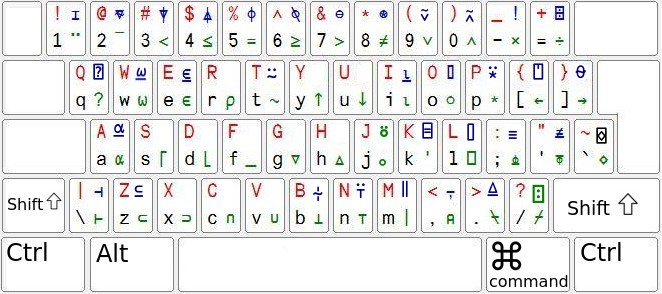
\includegraphics{figs/aplkb-largekeys.jpg}

\begin{lstlisting}[language=apl]
~/apl/apldocs$ rlwrap sbcl --noinform
CL-USER(1): (ql:quickload :april :silent t)
(:APRIL)
CL-USER(2): (load "src/rdapl.lisp")

T
CL-USER(6): @42 {⍺} 64 ⍝ left argument
42
42
CL-USER(7): @42 {⍵} 64 ⍝ right argument
64
64
\end{lstlisting}

\noindent
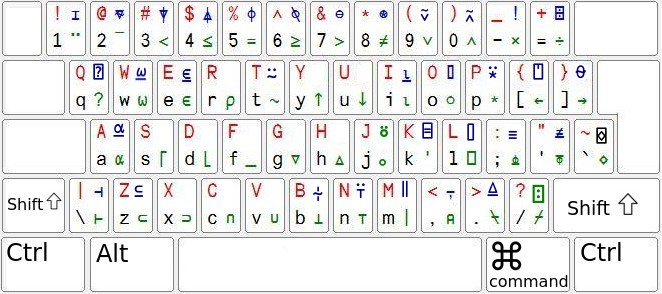
\includegraphics{figs/aplkb-largekeys.jpg}

\begin{lstlisting}[language=apl]
CL-USER(8): @42 ⌈ 64 ⍝ max
64
64
CL-USER(9): @42 ⌊ 64  ⍝ min
42
42
CL-USER(22): @×/ 1 2 3 4 5 ⍝ insert × between elements
120
120
CL-USER(23): @⍳12  ⍝ iota
1 2 3 4 5 6 7 8 9 10 11 12
#(1 2 3 4 5 6 7 8 9 10 11 12)
CL-USER(24): @3 4 ⍴ ⍳12  ⍝ reshape
1  2  3  4
5  6  7  8
9 10 11 12
#2A((1 2 3 4) (5 6 7 8) (9 10 11 12))
CL-USER(25): @+⌿ (3 4 ⍴ ⍳12)  ⍝ reduce colums
15 18 21 24
#(15 18 21 24)
CL-USER(26): @+/ (3 4 ⍴ ⍳12)  ⍝ reduce lines
10 26 42
#(10 26 42)
\end{lstlisting}

\chapter{Dyalog APL}\large
You may want to download a fully-featured commercial
APL to learn the language. In this case, I recommend
a free subscription to Dyalog APL.

In this chapter, I will focus on handling the
Dyalog system rather than teaching APL.
After all, you can learn APL through one
of the many tutorials available on the web.

After requesting a free subscription,
download and install the package.
Subsequently, initiate Dyalog APL by calling
its executable file from the terminal.
\begin{quote}
\verb|~/apl$ dyalog|
\end{quote}
\begin{figure}[!h]
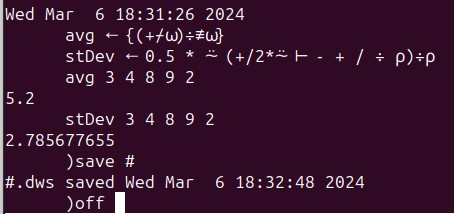
\includegraphics{figs/dyalog-save-ws.jpg}
\caption{Dyalog APL terminal}
\label{fig:dyalog-save-ws}
\end{figure}

In Figure~\ref{fig:dyalog-save-ws}, I defined
 \verb|avg|, which calculates the
average of a vector, and \verb|stDev|, which
produces the standard deviation. After testing
these functions, I saved the root \verb|#| workspace.
Following that, I entered \verb|)off| to exit APL.

\newpage
Below is an APL keyboard. The four new APL
keys that haven't been covered are circled in red.

\verb||\\
\hspace*{-0.5cm}
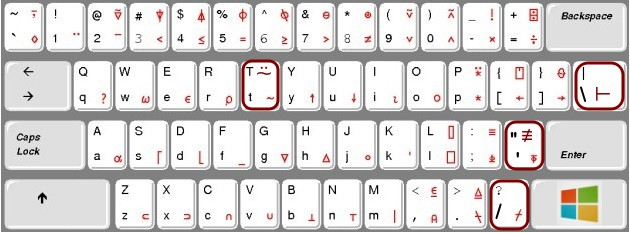
\includegraphics{figs/apl-aspas-barra-T.jpg}

The convention of using the sharp (\verb|#|)
character to represent the key sequence that
produces the APL symbols is reiterated in the
following figure for easy reference.

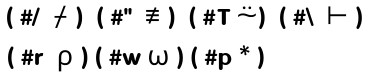
\includegraphics{figs/sharp-trwp.jpg}

The next time I use the Dyalog ecosystem,
I can download the saved workspace and
utilize the \verb|avg| and \verb|stDev| functions.
\begin{quote}
  \verb|~/apl$ dyalog|
\end{quote}
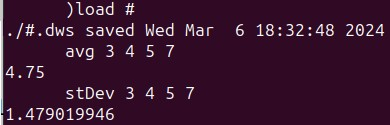
\includegraphics{figs/loadws.jpg}

\section{No source code in plain text}
APL was invented by the Canadian programmer Kenneth
Iverson well before the widespread availability
of text editors. Therefore, it provided its own
tools to edit functions and store them in the
so-called workspaces.

However, APL vendors have kept their
products {\em ``up to date''} by offering facilities
to deal with source code files in text format,
in a scheme not incompatible with workspaces.
In particular, the Link library distributed
with Dyalog APL allows linking directories
populated with text files to a workspace.

Let's place the text file \verb|stat.apl|
into the \verb|dsrc/| directory, as illustrated
in the figure~\ref{fig:stat}, page~\pageref{fig:stat}.

\begin{figure}[!h]
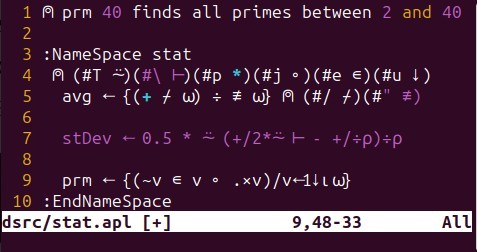
\includegraphics{figs/dsrc.jpg}
\caption{Source code of the stat workspace}
\label{fig:stat}
\end{figure}

I executed \verb|dyalog| from the \verb|aplf|
directory, which contains the subdirectory \verb|dsrc|.
\begin{quote}
\begin{verbatim}
~/aplf$ ls
dsrc
~/aplf$ dyalog
\end{verbatim}
\end{quote}

As seen in Figure~\ref{fig:link-import}, the
command \verb|]Link.import # dsrc| imported
the workspace defined in the file \verb|stat.apl|.

\begin{figure}[!h]
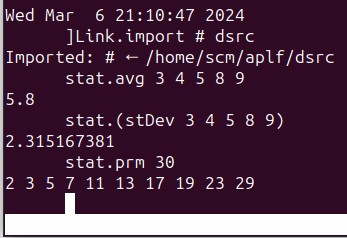
\includegraphics{figs/link-import.jpg}
\caption{]Link.import \# dsrc}
\label{fig:link-import}
\end{figure}

\begin{lstlisting}[language=apl]
     3 4 ⍴ ⍳12
1  2  3  4
5  6  7  8
9 10 11 12
      ≢ (3 4 ⍴ ⍳12)
3
\end{lstlisting}

\section{]Link.Create}
  When you enter a Dyalog session,
  you can create a link between the active
  workspace and a source directory.
\begin{lstlisting}[language=apl]
      ]Link.Create # dsrc                                           
Linked: # ←→ /home/scm/aplf/dsrc                                    
      stat.prm 30                                                   
2 3 5 7 11 13 17 19 23 29                                           
      ⎕ED 'dist' ⍝ Press Esc to quit editor
      3 4 5 6 dist 8 7 4 2
7.141428429
\end{lstlisting}
After linking \verb|dsrc| to the root
workspace \verb|#|, I tested the functions
and workspaces defined in \verb|dsrc|, namely,
the source code of the \verb|stat| workspace
listed in Figure~\ref{fig:stat} on page~\pageref{fig:stat}.
Finally, I used \verb|⎕ED 'dist'| to define
the function \verb|'dist'|, as shown
in Figure~\ref{srcfigs/edwindow.jpg} on
page~\pageref{srcfigs/edwindow.jpg}.

\begin{figure}[!t]
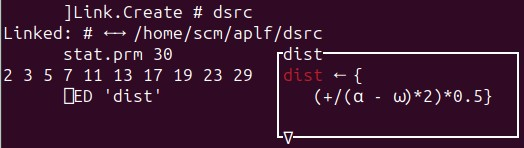
\includegraphics{srcfigs/edwindow.jpg}
\caption{⎕ED 'dist' -- Press Esc to quit}
  \label{srcfigs/edwindow.jpg}
\end{figure}
Then, I need to resync in order to store
the definition of figure~\ref{srcfigs/edwindow.jpg}
into \verb|dsrc|.
After that, I can leave Dyalog APL with \verb|)Off|.
\begin{verbatim}
      ]Link.Create # dsrc                                           
Linked: # ←→ /home/scm/aplf/dsrc                                    
      stat.prm 30                                                   
2 3 5 7 11 13 17 19 23 29                                           
      ⎕ED 'dist'  ⍝ Press Esc to quit editor                         
      3 4 5 7 dist 9 8 3 4
8.062257748
      ]Link.Resync dsrc -proceed
No action required
      )Off
\end{verbatim}
When I open a new session,
I just need to execute \verb|]Link.Create # dsrc| again
to recover all definitions stored in \verb|dsrc|.
By the way, when using an external editor
to populate a linked directory, you can place
only one function or workspace in each file.
\begin{verbatim}
      ]Link.Create # dsrc
Linked: # ←→ /home/scm/aplf/dsrc
      3 4 5 7 dist 9 8 3 4
8.062257748
      stat.prm 40
2 3 5 7 11 13 17 19 23 29 31 37
\end{verbatim}

\section{⎕ED}
Dyalog provides a structure editor for
defining functions. Here's how to request
the editing of the \verb|dist| function:
\begin{verbatim}
⎕ED 'dist' 
\end{verbatim}
When I start the editor, I get a window like
the one shown in Figure~\ref{srcfigs/edwindow.jpg}
on page~\pageref{srcfigs/edwindow.jpg}.
The \verb|Esc| key closes the current editor
window after saving any changes to the function
being edited. The main commands of the editor are:

\begin{itemize}
\item \verb|Ctrl-x j| -- toggles between the editor and the session.
\item \verb|Esc| closes the current window, having saved any changes.
\item \verb|Ctrl-x q| quits the editor.
\item \verb|Ctrl-x Ctrl x m| enters the resize loop.
  Arrows move the window around.
  \verb|PageUp|(or \verb|Ctrl-f|)
  and \verb|PageDown| (or \verb|Ctrl-h|)
  resize the window. Type \verb|Esc| to exit the resize loop.
\item \verb|Ctrl-x i| -- toggles insert mode.
\item \verb|Ctrl-x o| -- opens a new line.
\item \verb|Ctrl-x z| -- toggles the window to full size and back.
%\item \verb|Ctrl-x h| -- puts the cursor at the function id.
\item \verb|Ctrl-x t| plus arrows -- selects a region.
\item \verb|Ctrl-x c| -- copies the selected region or cursor line.
\item \verb|Ctrl-x l| -- toggles line numbering.
\item \verb|Ctrl-x ,| -- comments the cursor line.
\item \verb|Ctrl-x s| -- search.
\item \verb|Ctrl-x r| -- replace.
\end{itemize}

\section*{Keyboard practice}
\noindent
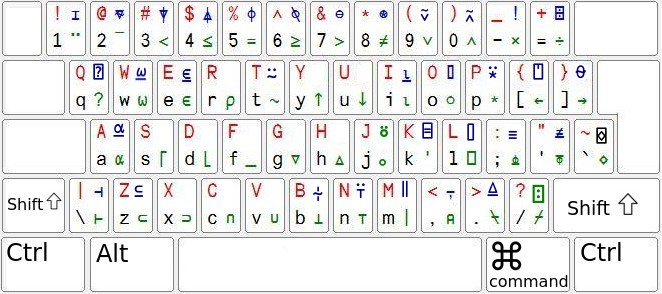
\includegraphics{figs/aplkb-largekeys.jpg}

\begin{lstlisting}[language=apl]
      fat ← { ⍵≤1: 1 ⋄ ⍵ × ∇⍵-1}
      fat 5
120
      42 + ¯12  ⍝ Prefix negative numbers with :cmd 2
30
      ∆x ← 0.001 ⍝ A nice way of writing small values 
      ∆x
0.001
     6 + ∘ ≢ 3 4 5 6 ⍝ X f∘g Y → X f (g Y)
10
     6 + (≢ 3 4 5 6)  
10
     herName ← 'Tati'
     howMany ← 8
     'Bugs Bunny ', (⍕howMany),' carrots.'
Bugs Bunny 8 carrots.
     'Hello, ', (⍕herName), '!'
Hello, Tati!
     'The factorial of 10 is ', (⍕ !10)
The factorial of 10 is 3628800     
\end{lstlisting}

\chapter{Tacit programming}

There are two ways of programming in APL
\begin{enumerate}
\item Direct function, or dfn
  \\ \verb|{(+/⍵) ÷ ⍴⍵} 3 4 5| $\rightarrow$ 4 ⍝ Average
\item Tacit programming\\
  \verb|(+/ ÷ ⍴) 3 4 5| $\rightarrow$ 4 ⍝ Tacit average
\end{enumerate}


\section{Direct function}

A direct function has the form \verb|{expr}|
where \verb|expr| is an APL expression
containing the parameters ⍺ and ⍵.
Here, the parameter ⍺ represents the left
argument, and the parameter ⍵ represents
the right argument.
\begin{lstlisting}[language=apl]
      {+/⍵ ÷ ⍴⍵} 3 4 5 8 9 ⍝ Average
5.8
      distance ← {(+/(⍺ - ⍵)*2)*0.5}
      3 4 5 distance 8 10 2
8.366600265
      42 {⍺} 64
42
      42 {⍵} 64
64
\end{lstlisting}

\section{Guards}
A guard is a boolean expression followed
by a colon and an APL expression.
The APL expression is calculated when
its associated guard is the first one
to evaluate to true.

A dfn may contain any number of guarded
expressions, each on a separate line.
When the guarded expressions
are on the same line, they must be separated
by ⋄ diamond symbols, obtained by
typing the \cmdkey\verb| ` | key sequence.

Direct functions use recursion in place of iteration.
Normally, a reference to the current function
is performed through the function’s name,
as in Lisp. However, anonymous
functions represent self-reference with
the ∇ symbol, typed with \cmdkey g.
\begin{verbatim}
      {⍵ < 0: -⍵ ⋄ ⍵ ≠ 0: ⍵ * 0.5} ¯42
42
      {⍵ < 0: -⍵ ⋄ ⍵ ≠ 0: ⍵ * 0.5} 0
      {⍵ < 0: -⍵ ⋄ ⍵ ≠ 0: ⍵ * 0.5} 64
8
      fib ← { 1 ≥ ⍵ : ⍵ ⋄ (fib ⍵ - 1) + (fib ⍵ - 2)}
      fib 5
5
      fib 6
8
      { ⍵ < 1 : 1 ⋄ ⍵ × ∇ ⍵ - 1} 6
720
\end{verbatim}
The last example calculates the
factorial of 6 recursively.
As it defines an anonymous function,
recursion is represented by the ∇ triangle symbol.


\section{Tacit programming}
In tacit programming, also called
point-free style, functions are defined
in terms of implicit arguments. This is in
contrast to the explicit use of arguments
in dfns (⍺ ⍵).

\begin{lstlisting}[language=apl]
      (+⌿÷≢) ⍳10   ⍝ Mean of the first ten integers
5.5
     (1 ∧ ⊢,÷)2.625
21 8
      21 ÷ 8 ⍝ Fraction
2.625
     (1 ∧ 0 1∘⊤,÷)2.625
2 5 8
     ○ 2
6.283185307
\end{lstlisting}


The following seven recursive rules
transform a dfn (definition with explicit
references to the left parameter ⍺ and
to the right parameter ⍵) into tacit
form (definition without explicit use of parameters):

\begin{description}
\item[fgh-fork] \verb|{X f Y} → ({X} f {Y})|
\item[gh-atop] \verb|{  f Y} → (    f {Y})|
\item[Agh-fork] \verb|{A f Y} → ( A  f {Y})|
\item[commute] \verb|{X f A} → (A(⊢f⊣) X)|
\item[left] \verb|{⍺} → ⊣|
\item[right] \verb|{⍵} → ⊢|
\item[constant] \verb|{A} → ((A)⊣⊣)|
\end{description}
where:
\begin{itemize}
  \item \verb|X| and \verb|Y| are value expressions
  with free occurrences of ⍺ or ⍵.

  \item \verb|A| is an expression
  without free occurrences of ⍺ or ⍵.

  \item \verb|f| is a functional expression
  with no occurrences of free ⍺ or ⍵.

  \item ⍺ and ⍵ are said to occur \emph{free}
  in an expression if they are not enclosed
  in curly braces. In the expression
  \verb|(⍺+2{⍺+⍵}3)|, ⍺ is free, but ⍵ is not.
\end{itemize}

I am reproducing below an example of conversion
from a dfn to tacit form that I found in a tutorial
on the Dyalog portal. My version includes some
small corrections. The subexpression that will
be converted at each step is enclosed within French quotes.
\begin{verbatim}
  «{(2+⍺)×⍵÷3}»            ⍝fgh-fork: {X f Y} to ({X} f {Y})
→ («{2+⍺}» × {⍵÷3})        ⍝Agh-fork: {A f Y} to ( A  f {Y})
→ ((2+«{⍺}»)×{⍵÷3})        ⍝left: {⍺} to ⊣
→ ((2+⊣) × «{⍵÷3}»)        ⍝commute: {X f A} to (A(⊢f⊣) X)
→ ((2+⊣) × «{3(⊢÷⊣)⍵}»)    ⍝Agh-fork: {A f Y} to ( A  f {Y})
→ ((2+⊣) × (3(⊢÷⊣) «{⍵}»)) ⍝right: {⍵} to ⊢
→ ((2+⊣)×(3(⊢÷⊣)⊢))        ⍝the tacit form
\end{verbatim}
\label{dfn-to-tacit}

Let's consider another example.
The function \verb|{(+⌿⍵)÷≢⍵}| calculates
the average of a vector, as illustrated below.
\begin{quote}
\begin{verbatim}
     {(+⌿⍵)÷≢⍵}  3 4 5 8 9
5.8
\end{verbatim}
\end{quote}
Let us apply the inference rules
to derive the tacit version.
\begin{verbatim}
«{+⌿⍵ ÷ ≢⍵}»              ⍝ {X f Y} to ({X} f {Y})
(«{+⌿⍵}» ÷ «{≢⍵}»)        ⍝ {f Y} to (f {Y})
((+⌿ «{⍵}») ÷ (≢ «{⍵}»))  ⍝ {⍵} to ⊢
((+⌿⊢) ÷ (≢ ⊢))
\end{verbatim}
The above program works; however, its
expression could be much simpler by applying
the rules in Figure~\ref{fig:simplification}.
\begin{quote}
\begin{verbatim}
      ((+⌿⊢) ÷ (≢ ⊢)) 3 4 5 8 9
5.8
\end{verbatim}
\end{quote}
By applying the rule \verb|(f⊢)g(h⊢) to (f g h)⊢|,
the expression \verb|((+⌿⊢) ÷ (≢ ⊢))|
becomes \verb|((+⌿)÷ ≢)⊢|. If we remove
the superfluous parentheses, we get the final
result \verb|((+⌿÷≢)⊢)| in tacit form.
The only function of the presence of \verb|⊢| in
the expression is to ignore an unwanted left argument.


\begin{figure}[!t]
\begin{verbatim}
(f⊢)g(h⊢) to (f g h)⊢  ⍝ ⊢ factoring
(f⊢)g ⊢   to (f g ⊢)⊢  ⍝ ⊢ factoring
⊣ g ⊢   to g           ⍝ dyadic function application
(f(g h)) to ((f g)h)   ⍝ association
\end{verbatim}
\caption{Simplification rules for tacit functions}
\label{fig:simplification}
\end{figure}

Below, you will find a test of the average
function, both in its dfn version and also
in the tacit version. Note that all steps
of the conversion to the tacit version
work as expected. The option \verb|-b|
suppresses the banner in a session.
\begin{verbatim}
~/aplf$ dyalog -b
     {(+⌿⍵)÷≢⍵} 3 4 5 8 9 ⍝ dfn
5.8
      ({+⌿⍵} ÷ {≢ ⍵}) 3 4 5 8 9
5.8
      ((+⌿⊢) ÷ (≢ ⊢)) 3 4 5 8 9
5.8
      42 ((+⌿÷≢)⊢) 3 4 5 8 9
5.8
      (+⌿÷≢) 3 4 5 8 9
5.8
\end{verbatim}
If you provide a left argument to the \verb|(+⌿÷≢)|
function, APL will generate an error.
However, in the \verb|((+⌿÷≢)⊢)| version,
the ⊢ operator will ignore the unwanted argument.

\section{]box}
  If you want a boxing display for your
  tacit functions, you can go to your session
  and type the commands below.
\begin{verbatim}
     ]Box ON -trains=box
Was OFF -trains=box
      (+⌿÷≢)
      ]box -trains=tree
Was -trains=tree
      (+⌿÷≢)
\end{verbatim}
The result is shown
in Figure~\ref{fig:boxon} below.
As you can see, the option \verb|-trains=tree| draws
a tree instead of a box.
\begin{figure}[!h]
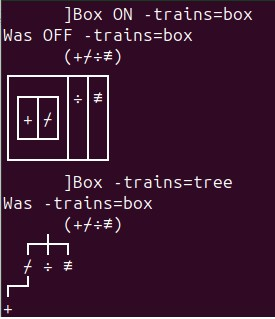
\includegraphics{srcfigs/boxon.jpg}
\caption{]box ON}
\label{fig:boxon}
\end{figure}

You can get help for \verb|]Box| by
typing \verb|]Box -??| during a session.
In particular, the help shows that there
are four options for \verb|-trains|, namely,
\verb|-trains=box|, \verb|-trains=tree|,
\verb|-trans=def| and \verb|-trains=parens|.
\begin{lstlisting}[language=apl]
      ]Box on -trains=def
Was OFF -trains=box
      (32∘+)∘(×∘1.8) ⍝ Fahrenheit from Celsius
32∘+∘(×∘1.8)
      32 ∘ + ∘ (×∘1.8) 100
212
\end{lstlisting}

\section{Tacit average}
Let us use the rules on page \pageref{dfn-to-tacit}
to transform the anonymous
function \verb|{+/⍵ ÷ ⍴⍵}|
into its tacit form.
\begin{verbatim}
«{+/⍵ ÷ ⍴⍵}»               ⍝ {X f Y} to ({X} f {Y})
(«{+/⍵}» ÷ «{⍴⍵}»)         ⍝ {f Y} to (f {Y})
(((+/)«{⍵}») ÷ (⍴ «{⍵}»))  ⍝ {⍵} to ⊢
(((+/)⊢) ÷ (⍴ ⊢))          ⍝ (f ⊢) g (h⊢) to (f g h) ⊢
((+/) ÷ ⍴) ⊢               ⍝ ⊢ ignores left argument
\end{verbatim}
Let us test both the explicit (defn)
expression and the tacit function.
You may also want to see what the tacit
function looks like in the \verb|]box ON| format.
\begin{quote}
\begin{verbatim}
     ((+/) ÷ ⍴) 3 4 5 8 9
5.8
      {+/⍵ ÷ ⍴⍵} 3 4 5 8 9
5.8
\end{verbatim}
\end{quote}

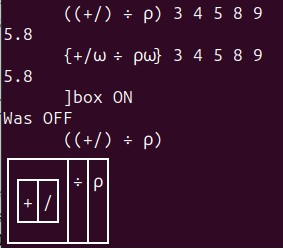
\includegraphics{srcfigs/avg-in-box-format}

\newpage
\section{Plots}
To access the Plot options,
type ]Plot -?? during a session.
  Below, you will find a few examples of plots.
\begin{verbatim}
]Plot (2 3 6 7 8 12 19)  (9 8 7 6 5 4 3) -type=XBar
\end{verbatim}
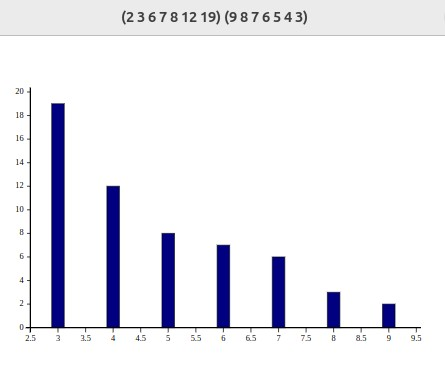
\includegraphics{srcfigs/kaplan-meyer-xbar.jpg}

\begin{verbatim}
]Plot (2 3 6 7 8 12 19)  (9 8 7 6 5 4 3) -type=Step
\end{verbatim}
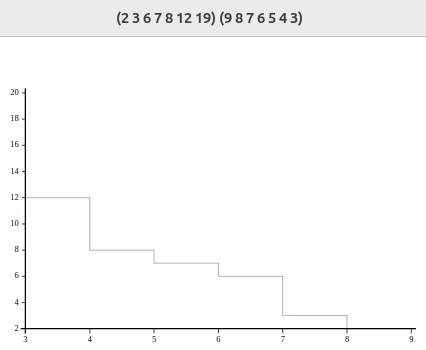
\includegraphics{srcfigs/kaplan-meyer-steps.jpg}

\newpage
\begin{verbatim}
]Plot (2 3 6 7 8 12 19)  (9 8 7 6 5 4 3) -type=Line
\end{verbatim}
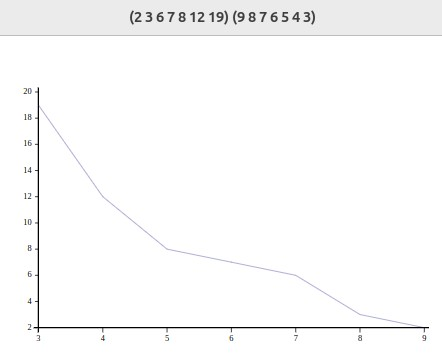
\includegraphics{srcfigs/kaplan-meyer-line.jpg}


\begin{verbatim}
]Plot (2 3 6 7 8 12 19)  (9 8 7 6 5 4 3) -type=Tower
\end{verbatim}
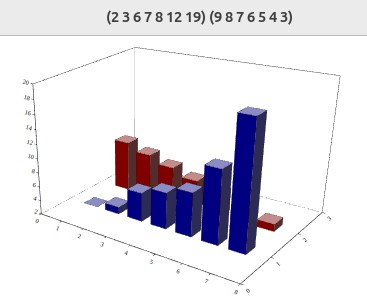
\includegraphics{srcfigs/kaplan-meyer-tower.jpg}

\chapter{Sockets}
\large
Let us explore how to receive
calculations in Python from Dyalog APL.
Start the Python interpreter and create
a socket assigned to the variable \verb|srv|.
\begin{verbatim}
~/apl/apldocs$ python -q
>>>> import socket
>>>> srv= socket.socket(socket.AF_INET, socket.SOCK_STREAM)
>>>> srv.bind(("localhost", 7342))
>>>> srv.listen()
>>>> client, address= srv.accept()
\end{verbatim}

\paragraph{APL Side.} Send messages.
\begin{lstlisting}[language=apl]
     )copy conga DRC
/opt/mdyalog/19.0/64/unicode/ws/conga.dws
      DRC.Init '' ⍝ Empty string
0  Conga loaded from: conga35_64.so
      DRC.Clt 'my socket' 'localhost' 7342 'Text'
0  my socket
      DRC.Send 'my socket' ('7!= ', ⍕(!7),⎕UCS 10)
0  my socket.Auto00000000
      DRC.Send 'my socket' (⍕ , (2 4 ⍴ ⍳ 8), ⎕UCS 10)
0  my socket.Auto00000001
\end{lstlisting}

\paragraph{Python Side.} Receive and decode message.
\begin{verbatim}
>>>> aplInput= client.recv(1024)
>>>> aplInput.decode("utf-8")
'7!= 5040 \n1 2 3 4 \n 5 6 7 8 \n'
>>>> print(aplInput.decode("utf-8"))
7!= 5040 
1 2 3 4 
 5 6 7 8 
\end{verbatim}

\section{Messages from Python}
Now, let's explore how to send messages from Python to APL.
\begin{verbatim}
~/apl/apldocs$ python -q
>>>> import socket
>>>> srv= socket.socket(socket.AF_INET, socket.SOCK_STREAM)
>>>> srv.bind(('localhost', 7342)) #Achtung: nested ((oJo))
>>>> srv.listen()
>>>> client, address= srv.accept() # Go to APL to Init conga
\end{verbatim}

\paragraph{APL side.} Create socket.
\begin{lstlisting}[language=apl]
     )copy conga DRC
/opt/mdyalog/19.0/64/unicode/ws/conga.dws
      DRC.Init ''
0  Conga loaded from: conga35_64.so
      DRC.Clt 'my socket' 'localhost' 7342 'Text'
0  my socket
      ⍝ At this point, python is free.
      ⍝ Type the command below, and go to
      ⍝ the Python side and send a message.
      DRC.Wait 'my socket' 999999
\end{lstlisting}

\paragraph{Python side.} Send the message.
\begin{verbatim}
>>>> client.send(b"Hello, Dyalog.")
37
\end{verbatim}

\paragraph{APL side.} Receive the message.
\begin{lstlisting}[language=apl]
      DRC.Wait 'my socket' 999999
      0  my socket  Block  Hello, Dyalog.
\end{lstlisting}

\newpage
\section{Second message from Python}
\begin{lstlisting}[language=apl]
      ⍝ Request a second message from Python.
      ⍝ Go to the Python side and send the       
      ⍝ second message. Dyalog is waiting.
      msg ← DRC.Wait 'my socket' 999999
\end{lstlisting}

\paragraph{Python side} sends a second message.
\begin{verbatim}
>>>> client.send(b"Second message from Python.")
36
\end{verbatim}

\paragraph{APL side.} The message is in a vector,
and the text is the fourth element.
\begin{lstlisting}[language=apl]
      msg ← DRC.Wait 'my socket' 999999
      ⍝ The message is stored in the variable msg
      msg
0  my socket  Block  Second message from Python.
      msg[4]  ⍝ It is the 4th element of array msg
 Second message from Python.
\end{lstlisting}



\end{document}

